\documentclass[aspectratio=169,12pt]{beamer}

% ---------------------------------------------------------------------------
% Short research update (about 30 min) for the lab that collected the data.
% Shortened from ../Presentation_ABC: fewer words and numbers, figures reused
% from the models' plot folders. Compile from this folder: pdflatex
% Presentation.tex (twice). amplitude_schedule.png is made by
% Make_Amplitude_Schedule.py.
% ---------------------------------------------------------------------------

\usepackage{amsmath}
\usepackage{amssymb}
\usepackage{booktabs}
\usepackage{graphicx}
\usepackage{tikz}
\usetikzlibrary{decorations.pathmorphing,positioning,arrows.meta,calc}

% ---- style: as in Presentation_ABC -----------------------------------------
\usetheme{default}
\definecolor{plotblue}{HTML}{2A78D6}
\definecolor{plotorange}{HTML}{EB6834}
\definecolor{plotred}{HTML}{E34948}
\definecolor{ink}{HTML}{0B0B0B}
\definecolor{muted}{HTML}{52514E}
\setbeamercolor{frametitle}{fg=plotblue}
\setbeamercolor{title}{fg=plotblue}
\setbeamercolor{structure}{fg=plotblue}
\setbeamercolor{normal text}{fg=ink}
\setbeamerfont{frametitle}{series=\bfseries}
\setbeamertemplate{navigation symbols}{}
\setbeamertemplate{itemize items}[circle]
\setbeamertemplate{footline}{%
  \hfill{\color{muted}\scriptsize\insertframenumber/\inserttotalframenumber}\hspace{1em}\vspace{0.6em}}

% ---- figure folders ----------------------------------------------------------
\newcommand{\plotsA}{../Model_A/Plots_A}
\newcommand{\plotsB}{../Model_B/Plots_B}
\newcommand{\plotsC}{../Model_C/Plots_C}

% a frame with one figure as large as fits and a one-line takeaway under it; the
% figure's own title is cropped off (the analysis PNGs are 200 dpi with the title in
% the top 61 px = 22 bp)
\newcommand{\takeframe}[3]{%
  \begin{frame}{#1}
    \centering
    \includegraphics[width=\textwidth,height=0.74\textheight,keepaspectratio,
                     trim=0 0 0 22bp,clip]{#2}
    \par\vspace{0.3em}{\small #3}
  \end{frame}}

% ---- trial schematic (slide "The task: one trial") -------------------------
\tikzset{
  handline/.style={line width=1.1pt, line join=round, draw=muted},
  stimprobe/.style={line width=1.3pt, draw=plotblue, decorate,
    decoration={zigzag, amplitude=2.6mm, segment length=3.2mm,
                pre length=5.5mm, post length=5.5mm}},
  distprobe/.style={line width=1.3pt, draw=plotorange, decorate,
    decoration={zigzag, amplitude=1mm, segment length=1.1mm,
                pre length=5mm, post length=5mm}},
  noprobe/.style={line width=1.3pt, draw=plotorange},
  handstroke/.style={handline, fill=white},
  handfill/.style={fill=white},
}
% an open hand, fingers up, at (#1); #2 = 1 (thumb left) or -1 (thumb right); #3 = palm label
\newcommand{\trialhand}[3]{%
  \begin{scope}[shift={(#1)}, scale=1.35]
    \begin{scope}[xscale=#2]
      \clip (-1.5,-0.62) rectangle (1.5,2);
      % outline of the union: stroke every part, then fill every part on top
      \foreach \opt in {handstroke, handfill} {
        \foreach \x/\h in {-0.3/1.25, -0.1/1.42, 0.1/1.36, 0.3/1.15}
          \path[\opt, rounded corners=2.6pt] (\x-0.085,0.4) rectangle (\x+0.085,\h);
        \path[\opt, rotate around={38:(-0.33,0.1)}, rounded corners=2.6pt]
          (-0.42,0.05) rectangle (-0.24,0.78);
        \path[\opt, rounded corners=5pt] (-0.4,-0.05) rectangle (0.4,0.62);
        \path[\opt] (-0.3,-0.8) rectangle (0.3,0.1);
      }
    \end{scope}
    \node[font=\scriptsize, muted] at (0,0.22) {#3};
  \end{scope}}
% one trial panel at x-offset #1; #2 = 1 for bimanual (distractor on), 0 for unimanual
\newcommand{\trialpanel}[2]{%
  \begin{scope}[shift={(#1,0)}]
    \trialhand{0,0}{1}{stim}
    \trialhand{2.6,0}{-1}{dist}
    \draw[stimprobe] (0,2.1) -- (0,4.6);
    \node[plotblue, left] at (-0.35,3.35) {$x_\text{stim}$};
    \ifnum#2=1
      \draw[distprobe] (2.6,2.1) -- (2.6,4.6);
      \node[plotorange, right] at (2.85,3.35) {$x_\text{d}$};
      \node[align=center, font=\small\bfseries] at (1.3,5.35)
        {bimanual trial\\[-1pt]{\normalfont\scriptsize\color{muted}(with distractor)}};
    \else
      \draw[noprobe] (2.6,2.1) -- (2.6,4.6);
      \node[plotorange, right] at (2.7,3.35) {$x_\text{d} = 0$};
      \node[align=center, font=\small\bfseries] at (1.3,5.35)
        {unimanual trial\\[-1pt]{\normalfont\scriptsize\color{muted}(no distractor)}};
    \fi
  \end{scope}}


% ---- title ---------------------------------------------------------------------
\title{How a Distractor on One Hand Changes Judgments on the Other}
\subtitle{Research update}
\author{Vera Schroeder}
\date{November 2026}

\begin{document}

\begin{frame}
  \titlepage
\end{frame}

% !TEX root = ../Presentation.tex
% ---------------------------------------------------------------------------
% Plan of the talk and the terms used for the data
% ---------------------------------------------------------------------------
\section{Terms}

\begin{frame}{Today}
  \Large
  \begin{enumerate}
    \item The terms I use for the data
    \item Three models of the data
    \item What they show
    \item Open questions for you
  \end{enumerate}
\end{frame}

\begin{frame}{Two kinds of trial}
  \centering
  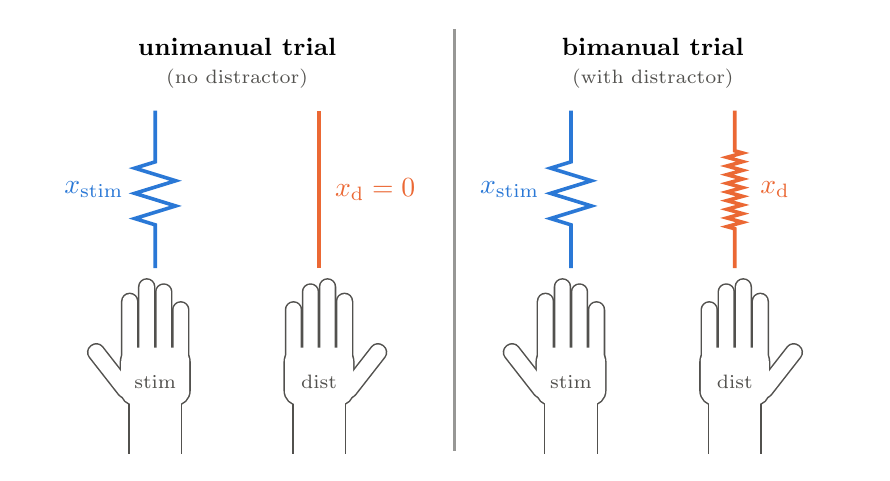
\begin{tikzpicture}[scale=0.8, every node/.append style={transform shape=false}]
    \trialpanel{0}{0}
    \draw[muted!60, line width=0.8pt] (4.75,-0.8) -- (4.75,5.9);
    \trialpanel{6.6}{1}
  \end{tikzpicture}
  \par\vspace{0.4em}
  \textbf{Group:} hand $\times$ trial type, so four groups: left/right, unimanual/bimanual
\end{frame}

\begin{frame}{Each session has one distractor amplitude}
  \centering
  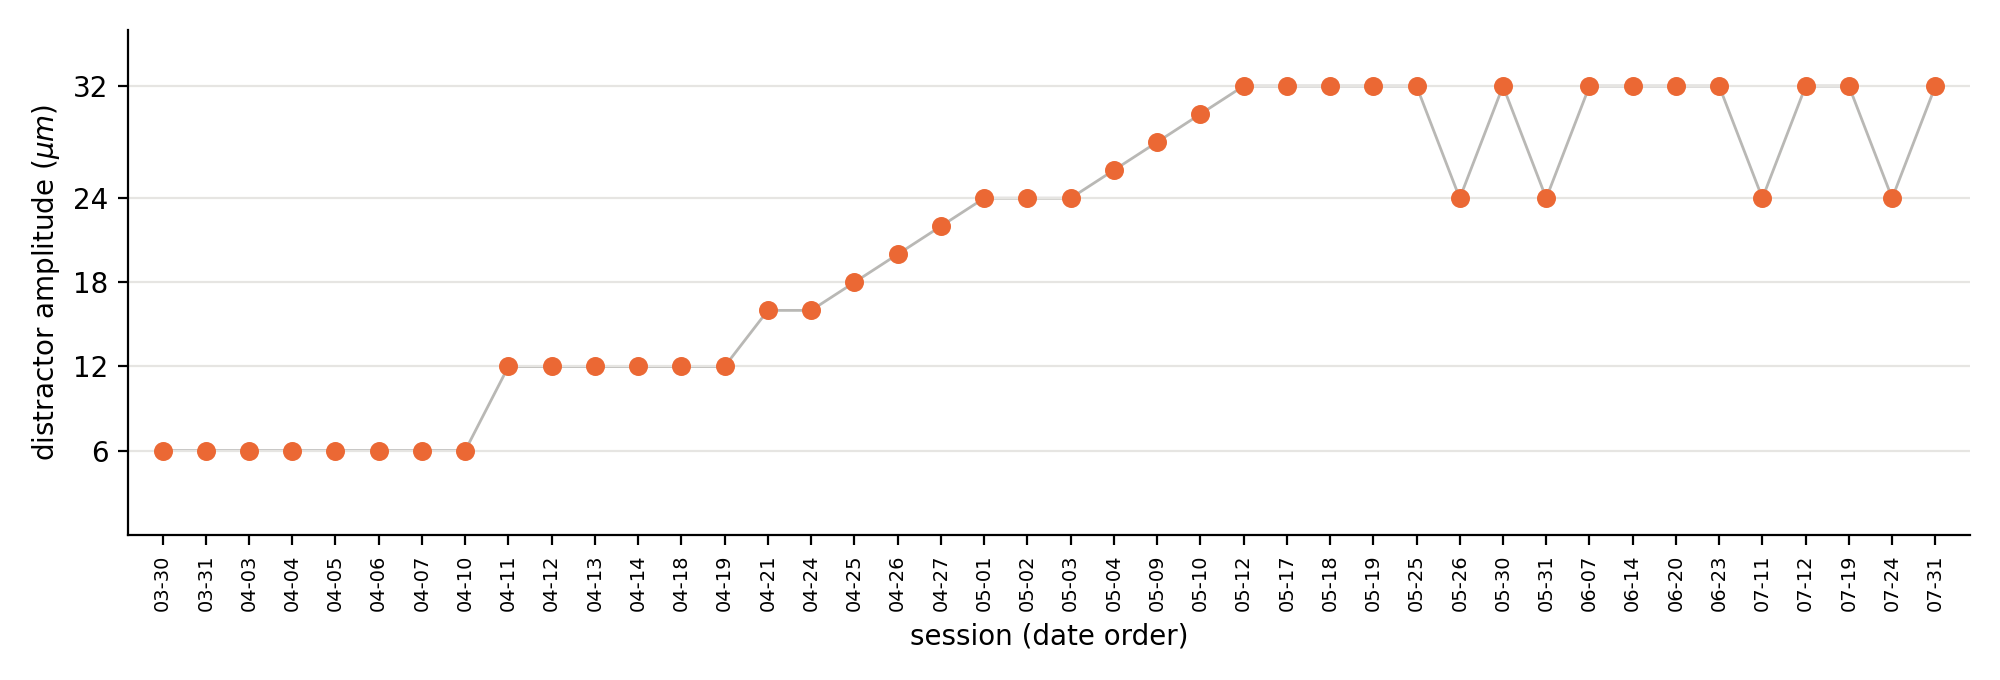
\includegraphics[width=\textwidth]{amplitude_schedule.png}
  \par\vspace{0.3em}
  42 sessions of about 300 trials, from one monkey (Sirius)
\end{frame}

\begin{frame}{The psychometric curve}
  \begin{columns}[c]
    \begin{column}{0.52\textwidth}
      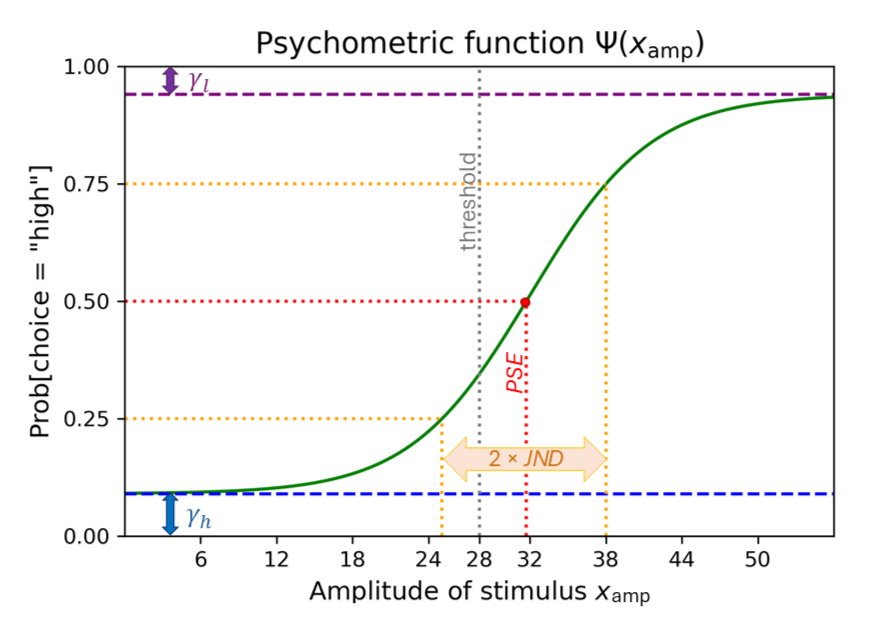
\includegraphics[width=\textwidth]{../Presentation_ABC/example_psych_func.png}
    \end{column}
    \begin{column}{0.46\textwidth}
      \small
      \begin{itemize}
        \setlength{\itemsep}{0.5em}
        \item \textbf{PSE} (bias): called ``high'' half the time\\
              {\color{muted}lower PSE = more ``high'' answers}
        \item \textbf{JND} (sensitivity): how fast the curve rises\\
              {\color{muted}larger JND = less precise}
        \item \textbf{Lapses:} answers the stimulus does not explain\\
              {\color{muted}${\color{blue}\gamma_h}$ = floor, ${\color{purple}\gamma_l}$ = gap below the ceiling}
      \end{itemize}
    \end{column}
  \end{columns}
  \vspace{0.5em}
  \centering
  \textbf{Distractor effect} = bimanual $-$ unimanual, for each hand
\end{frame}

% !TEX root = ../Presentation.tex
% ---------------------------------------------------------------------------
% The three models and how they are checked
% ---------------------------------------------------------------------------
\section{Models}

\begin{frame}{Three models}
  \begin{itemize}
    \setlength{\itemsep}{1em}
    \item \textbf{Model A:} one curve per group, all sessions pooled
    \item \textbf{Model B:} a curve for every session\\
          {\color{muted}sessions may differ, but are assumed to resemble each other}
    \item \textbf{Model C:} like B, but the distractor's shift is proportional to its
          amplitude\\
          {\color{muted}one curve per hand, with both trial types}
  \end{itemize}
\end{frame}

\begin{frame}{How I check a model}
  \begin{enumerate}
    \setlength{\itemsep}{1em}
    \item \textbf{Simulated data:} make data with known answers, and check that the model
          gets them back
    \item \textbf{Real data:} check that the fitted model reproduces what the monkey did
    \item \textbf{Compare models:} how well each predicts trials left out of its fit
  \end{enumerate}
\end{frame}

% !TEX root = ../Presentation.tex
% ---------------------------------------------------------------------------
% Findings, from the Fit and model comparison reports of Models A, B and C
% ---------------------------------------------------------------------------
\section{Findings}

\begin{frame}{The distractor makes ``high'' answers more likely}
  \centering
  \includegraphics[width=0.46\textwidth]{\plotsA/Fit_Plots_A/curves_left.png}\hfill
  \includegraphics[width=0.46\textwidth]{\plotsA/Fit_Plots_A/curves_right.png}
  \par\vspace{0.3em}
  The bimanual curve (red) moves left: PSE about 4~$\mu m$ lower (left hand), 6~$\mu m$ (right)
\end{frame}

\takeframe{The shift appears in nearly every session}
  {\plotsB/Fit_Plots_B/effect_PSE_by_session.png}
  {One session per point, in date order (Model B). Below 0: the distractor lowers the PSE}

\takeframe{The shift grows with the distractor's amplitude}
  {\plotsC/Fit_Plots_C/pse_shift_vs_amplitude.png}
  {One session per point (Model C). But amplitude also rose over time}

% the circles mark the weakest stimuli (6 and 12 um) on curves_left/right.png, in
% coordinates relative to the image (0,0 = lower left, 1,1 = upper right)
\newcommand{\floorcurves}[1]{%
  \begin{tikzpicture}
    \node[anchor=south west, inner sep=0] (img) at (0,0)
      {\includegraphics[width=0.48\textwidth]{#1}};
    \begin{scope}[x={(img.south east)}, y={(img.north west)}]
      \draw[plotorange, line width=1.5pt] (0.21,0.205) ellipse (0.095 and 0.05);
    \end{scope}
  \end{tikzpicture}}

\begin{frame}{A floor under the bimanual curve}
  \centering
  \floorcurves{\plotsA/Fit_Plots_A/curves_left.png}\hfill
  \floorcurves{\plotsA/Fit_Plots_A/curves_right.png}
  \par\vspace{0.3em}
  With a distractor, the monkey sometimes answers ``high'' to the weakest stimuli
\end{frame}

\begin{frame}{Less clear}
  \begin{itemize}
    \setlength{\itemsep}{1em}
    \item \textbf{Sensitivity:} the left-hand JND is slightly larger with a distractor\\
          {\color{muted}driven by a few sessions; may be the same extra ``high'' answers}
    \item \textbf{Weak distractors:} on the right hand, a 6~$\mu m$ distractor shifts the
          PSE more than its amplitude predicts\\
          {\color{muted}not yet shown to matter for prediction}
  \end{itemize}
\end{frame}

% elpd differences from Model_B/Fit_B_Report.tex and Model_C/Fit_C_Report.tex
\begin{frame}{Which model predicts best?}
  \centering
  How much worse than Model B each model predicts left-out trials\\[0.3em]
  {\small\color{muted}(difference in log predictive score)}
  \par\vspace{1em}
  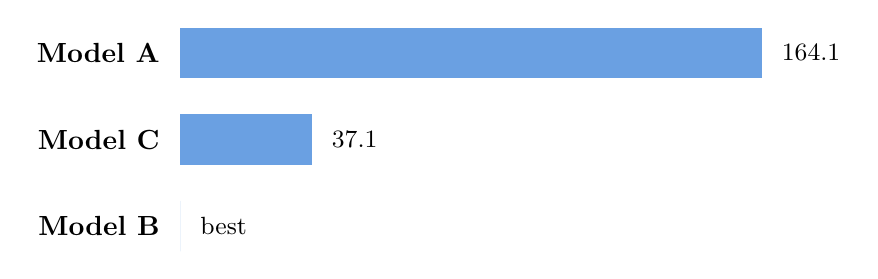
\begin{tikzpicture}[x=0.045cm]
    \foreach \m/\v/\y in {A/164.1/0, C/37.1/-1.1, B/0/-2.2} {
      \node[anchor=east, font=\bfseries] at (-3,\y) {Model \m};
      \fill[plotblue!70] (0,\y-0.32) rectangle (\v,\y+0.32);
      \node[anchor=west, font=\small] at (\v+3,\y) {\ifdim\v pt=0pt best\else\v\fi};
    }
  \end{tikzpicture}
  \par\vspace{1em}
  \raggedright
  \begin{itemize}
    \item B $\gg$ A: sessions really differ
    \item B $>$ C: C has one floor for both trial types
  \end{itemize}
\end{frame}

% the bimanual row of ppc_pooled_by_stimulus.png: 1223 px tall at 200 dpi, row starts at
% 600 px = 216 bp from the top
\begin{frame}{Why Model C falls short}
  \centering
  \includegraphics[width=0.85\textwidth,trim=0 0 0 216bp,clip]
    {\plotsC/Fit_Plots_C/ppc_pooled_by_stimulus.png}
  \par\vspace{0.3em}
  {\small Black: observed. Blue: Model C's prediction.}\\
  On bimanual trials, C predicts too few ``high'' answers to the weakest stimuli
\end{frame}

\begin{frame}{Summary}
  \begin{itemize}
    \setlength{\itemsep}{0.8em}
    \item The distractor lowers the PSE: about 4~$\mu m$ (left hand) and 6~$\mu m$ (right),
          in all three models
    \item The shift is larger in sessions with a stronger distractor
    \item With a distractor, the monkey sometimes answers ``high'' to the weakest stimuli
    \item Sessions differ, so each session needs its own curve
  \end{itemize}
\end{frame}

% !TEX root = ../Presentation.tex
% ---------------------------------------------------------------------------
% Questions for discussion and next steps
% ---------------------------------------------------------------------------
\section{Next}

\begin{frame}{Questions for you}
  \begin{enumerate}
    \setlength{\itemsep}{1.2em}
    \item \textbf{The extra ``high'' answers:} they seem to cluster in sessions with a strong
          distractor (being checked). Could the monkey sometimes respond to the distractor
          hand?
    \item \textbf{Amplitude and time:} the distractor amplitude rose over the sessions, so a
          growing effect could also be training or adaptation. Was the schedule chosen for a
          reason? Did anything else change over those months?
  \end{enumerate}
\end{frame}

\begin{frame}{Next steps}
  \begin{itemize}
    \setlength{\itemsep}{1em}
    \item \textbf{Model D:} separate lapse rates for unimanual and bimanual trials
    \item Test whether the bimanual lapse rate depends on the distractor amplitude, or on time
    \item Check Model D on simulated data before fitting the real data
  \end{itemize}
\end{frame}


\end{document}
